\documentclass[9pt,a4paper]{extarticle}

\usepackage[margin=12.5mm,top=11mm,bottom=12mm,headsep=3mm,footskip=6mm]{geometry}
\usepackage{fontspec}
\usepackage{kotex}
\usepackage{microtype}
\usepackage{multicol}
\usepackage{amsmath,amssymb}
\usepackage{booktabs,tabularx,array}
\usepackage{enumitem}
\usepackage{titlesec}
\usepackage{fancyhdr}
\usepackage{tikz}
\usetikzlibrary{arrows.meta,positioning}
\usepackage{pgfplots}
\pgfplotsset{compat=1.18}
\usepackage[hidelinks,bookmarks=false]{hyperref}
\usepackage{url}

\IfFontExistsTF{TeX Gyre Termes}{\setmainfont{TeX Gyre Termes}}{}
\IfFontExistsTF{TeX Gyre Heros}{\setsansfont{TeX Gyre Heros}}{}
\IfFontExistsTF{Noto Serif CJK KR}
  {\setmainhangulfont{Noto Serif CJK KR}}
  {\setmainhangulfont{Batang}}
\IfFontExistsTF{Noto Sans CJK KR}
  {\setsanshangulfont{Noto Sans CJK KR}}
  {\setsanshangulfont{Malgun Gothic}[BoldFont={Malgun Gothic Bold}]}
\renewcommand{\bfdefault}{b}

\definecolor{graphblue}{RGB}{28,92,158}
\definecolor{graphorange}{RGB}{207,95,27}

\setlength{\parindent}{0pt}
\setlength{\parskip}{2.4pt}
\setlength{\columnsep}{5mm}
\setlength{\columnseprule}{0pt}
\setlist[itemize]{leftmargin=1.25em,itemsep=0.5pt,topsep=1.5pt,parsep=0pt}
\setlist[enumerate]{leftmargin=1.4em,itemsep=0.5pt,topsep=1.5pt,parsep=0pt}
\setlength{\tabcolsep}{3.2pt}
\renewcommand{\arraystretch}{1.08}
\raggedcolumns
\emergencystretch=1em

\titleformat{\section}{\sffamily\bfseries\large}{\thesection.}{0.45em}{}
\titleformat{\subsection}{\sffamily\bfseries\normalsize}{\thesubsection}{0.4em}{}
\titlespacing*{\section}{0pt}{3.5pt}{2pt}
\titlespacing*{\subsection}{0pt}{2.8pt}{1pt}

\pagestyle{fancy}
\fancyhf{}
\fancyhead[L]{\sffamily\scriptsize SNU AI Challenge 2026}
\fancyhead[R]{\sffamily\scriptsize 순열 좌표계의 등변 학습과 최소 완전균형 추론}
\fancyfoot[C]{\sffamily\scriptsize \thepage}
\renewcommand{\headrulewidth}{0.35pt}
\renewcommand{\footrulewidth}{0pt}

\newcommand{\metric}[2]{%
  \begin{minipage}[t]{0.48\linewidth}
    {\sffamily\bfseries\large #1}\par
    {\scriptsize #2}
  \end{minipage}}
\newcommand{\code}[1]{\texttt{\footnotesize #1}}
\newcommand{\tightnote}[1]{{\scriptsize #1}}
\newcommand{\evidA}{\textsf{\scriptsize A}}
\newcommand{\evidB}{\textsf{\scriptsize B}}
\newcommand{\evidC}{\textsf{\scriptsize C}}
\newcolumntype{Y}{>{\raggedright\arraybackslash}X}
\newcolumntype{C}[1]{>{\centering\arraybackslash}p{#1}}
\newcolumntype{R}[1]{>{\raggedleft\arraybackslash}p{#1}}

\begin{document}
\thispagestyle{empty}

{\sffamily\bfseries\fontsize{17}{19}\selectfont
순열 좌표계의 등변 학습과 최소 완전균형 추론\par}
\vspace{2pt}
{\sffamily\fontsize{11}{13}\selectfont
24\,GB 환경의 Qwen3.6--27B 기반 4-프레임 시간 순서 복원\par}
\vspace{5pt}
\begin{tabularx}{\textwidth}{@{}Y r@{}}
\textbf{SNUAICHAL} · 대표 한지후 &
\href{https://github.com/SNUAICHAL/SNUAICHAL}{github.com/SNUAICHAL/SNUAICHAL}\\
\end{tabularx}
\vspace{2pt}\hrule\vspace{5pt}

\textbf{초록.}
본 과제는 문장과 무작위 순서의 네 이미지로 원래 시간 순서를 복원하는
4-순열 exact-match 문제다. 입력 순서를 바꾸면 출력의 좌표계도 함께 바뀐다는 점을
핵심 구조로 보고, (i) 결정론적 index-shuffle과 정답 변환으로 학습 좌표를
정렬하고, (ii) 각 view의 예측을 원래 slot 좌표로 역변환하며, (iii) 각 이미지가
각 표시 위치에 정확히 한 번 등장하는 최소 완전균형 Latin4로 집계했다.
Qwen3.6--27B를 rank-32 QLoRA로 학습한 checkpoint-2726은 단일 RTX~3090에서
NF4로 실행되었고 Public 0.93542를 기록했다. 같은 checkpoint의 confidence
tie-break(0.92670)과 24-view hard vote(0.93193), 더 긴 checkpoint-3400의
12-view hard vote(0.93542)를 함께 공개한다. 결과는 ``더 큰 계산''보다
\textbf{좌표 일관성, 최소 균형, 단순 집계}가 이 문제에서 중요함을 보인다.

\vspace{3pt}
\begin{multicols}{2}
\section{문제와 평가 관점}

입력은 문장 $s$와 이미지 $(x_1,x_2,x_3,x_4)$, 출력은
$S_4$의 원소다. 위치 하나만 틀려도 오답이므로 pairwise 단서뿐 아니라 네 장의
전역적 일관성이 필요하다. 또 동일한 네 장을 다른 순서로 보여 주면 정답 표기도
함께 변한다. 이를 무시한 단순 TTA는 서로 다른 좌표계의 숫자를 투표하는 오류를
만든다.

최종 평가는 Public뿐 아니라 Private, 코드 재현성, 보고서와 외부 데이터
일반화를 함께 고려한다. 따라서 Public 반복 제출에서 얻은 관찰은
\textbf{operational evidence}로만 쓰고 Private 성능의 보장으로 과장하지 않았다.

\subsection*{최종 시스템}
\begin{center}
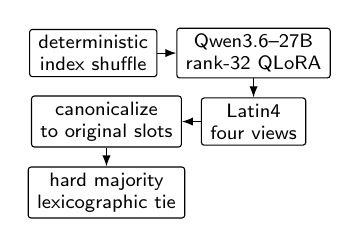
\begin{tikzpicture}[
  node distance=2.4mm,
  box/.style={draw,rounded corners=1pt,align=center,inner xsep=3.2pt,inner ysep=2.1pt,
              font=\sffamily\scriptsize},
  arr/.style={-{Latex[length=1.4mm]},thin}
]
\node[box] (a) {deterministic\\index shuffle};
\node[box,right=of a] (b) {Qwen3.6--27B\\rank-32 QLoRA};
\node[box,below=of b] (c) {Latin4\\four views};
\node[box,left=of c] (d) {canonicalize\\to original slots};
\node[box,below=of d] (e) {hard majority\\lexicographic tie};
\draw[arr] (a)--(b);
\draw[arr] (b)--(c);
\draw[arr] (c)--(d);
\draw[arr] (d)--(e);
\end{tikzpicture}
\end{center}

\subsection*{동결된 최종 계약}
\begin{tabularx}{\linewidth}{@{}lY@{}}
\toprule
Base & Qwen/Qwen3.6--27B, pinned revision\\
학습 & 9,535행, step 2,726 (2.28694 epochs)\\
Adapter & QLoRA $r/\alpha=32/32$, dropout 0.05\\
추론 & NF4, BF16 compute, SDPA, 512, batch 1\\
생성 & seed 42, thinking off, 64 tokens\\
TTA & 1234, 2341, 3412, 4123\\
집계 & hard majority; exact tie는 사전식 최소\\
\bottomrule
\end{tabularx}

\columnbreak
\section{핵심 기여}

\begin{enumerate}
\item \textbf{순열-등변 좌표 처리.}
학습의 Answer 변환과 추론의 역변환을 하나의 permutation algebra로 통일했다.
\item \textbf{최소 완전균형 TTA.}
네 cyclic view만으로 frame--position 노출 행렬을 정확히 균형화했다.
\item \textbf{실패까지 포함한 선택 근거.}
confidence 집계, 24-view, 추가 step이 악화 또는 무이득이었던 결과를 숨기지 않고
최종 단순화의 근거로 삼았다.
\item \textbf{24\,GB 실배치.}
27B base를 unmerged NF4로 유지해 단일 RTX~3090에서 실행하고, NVML로
process 밖 물리 peak를 측정했다.
\item \textbf{byte-level 재현성.}
base tree, adapter, command, source, image tree, raw output, CSV를 SHA-256
receipt로 연결했다.
\end{enumerate}

\subsection*{대표 결과}
\vspace{1pt}
\noindent
\metric{0.93542}{최종 Public score}\hfill
\metric{4 views}{완전균형 Latin4}\par\vspace{4pt}
\metric{0 / 3,276}{view parse failures}\hfill
\metric{21.15 GiB}{실측 physical peak}\par\vspace{4pt}
\metric{16.47 s}{generation / row}\hfill
\metric{3.89 h}{819행 end-to-end}

\subsection*{증거 등급}
\tightnote{\evidA\ = 동일 final pipeline의 제출·raw artifact,\quad
\evidB\ = 분리된 개발용 labeled 검증,\quad
\evidC\ = 수학·시스템 gate. 서로 다른 등급을 인과 비교로 합치지 않는다.}

\subsection*{한 문장 요약}
\textbf{가장 많은 view가 아니라, 원래 좌표로 정확히 되돌린 최소 균형 view가
더 정확하고 더 싸며 더 재현 가능했다.}

\subsection*{문제 구조와 설계 응답}
\begin{tabularx}{\linewidth}{@{}Y Y@{}}
\toprule
구조적 위험 & 대응\\
\midrule
입력 slot이 임의적 & index-shuffle + Answer 변환\\
view마다 label 좌표가 다름 & original-slot canonicalization\\
position exposure 편향 & Latin4의 $N(i,j)=1$\\
confidence가 미보정 & pure hard majority\\
24\,GB 단일 GPU & NF4, unmerged adapter, batch 1\\
검증 실행과 제출 불일치 & source·command·CSV hash chain\\
\bottomrule
\end{tabularx}

\subsection*{선택 원칙}
\begin{itemize}
\item 최고점이 동률이면 더 이른 checkpoint, 더 적은 view, 더 단순한 규칙을 택한다.
\item 동일하지 않은 model·split·checkpoint 비교는 결합 효과로 표시한다.
\item test label이 없으면 semantic 오류나 Private 개선을 추정하지 않는다.
\item 실패한 실험과 미실행 ablation도 명시해 선택 편향을 드러낸다.
\end{itemize}

\end{multicols}

\newpage
\section{데이터 활용과 학습}
\begin{multicols}{2}

\subsection{결정론적 index-shuffle}

고정 slot 학습은 내용 대신 위치 prior를 학습할 수 있다. 각
$(\text{seed},\text{epoch},\text{Id})$를 SHA-256으로 hash해 permutation
$g\in S_4$를 정하고 이미지와 Answer를 동시에 변환했다. 동일 seed와 데이터는
항상 동일한 view를 만들며, test-time canonicalization과 같은 좌표 규칙을 쓴다.

원래 Answer를 $y=(y_1,\ldots,y_4)$, displayed slot $j$에 놓인 원본 index를
$g_j$라 하면 학습 label은
\[
  T_g(y)_j = y_{g_j}.
\]
추론 출력 $p$를 원본 slot로 되돌리는 연산은
\[
  C_g(p)_{g_j}=p_j,\qquad C_g(T_g(y))=y.
\]
두 식의 round-trip을 단위 테스트로 고정했다.

\subsection{QLoRA 학습 계약}

Qwen3.6--27B의 vision-language prior를 유지하면서 24\,GB 추론을 가능하게 하려고
4-bit QLoRA를 적용했다. vision encoder는 고정하고 language의
\code{q/k/v/o}와 \code{gate/up/down} projection에 rank-32 adapter를
학습했다. 핵심 설정은 다음과 같다.

\begin{tabularx}{\linewidth}{@{}lY@{}}
\toprule
항목 & 설정\\
\midrule
Horizon & 3 epochs, final 2.28694\\
Learning rate & $10^{-4}$, cosine schedule\\
Batch & 1, gradient accumulation 8\\
Precision & NF4 base, BF16 compute\\
Image budget & 512$\times$512 상당\\
Seed & 42\\
Checkpoint & global step 2,726\\
\bottomrule
\end{tabularx}

최종 adapter의 512 tensor는 모두 finite였다. base는 merge/dequantize하지 않아
배포 메모리와 artifact 크기를 낮췄다.

\subsection{데이터 경계}

최종 Q36은 제공된 labeled 9,535행 전체를 학습했다. 따라서 같은 행을 사후
holdout처럼 채점하면 누수이며 최종 모델 선택 근거로 쓰지 않았다. 초기
Qwen3-VL--8B 단계의 image-disjoint clean954는 augmentation, parser와
checkpoint trend를 개발하는 \evidB\ surrogate였다. 최종 Q36의 수치는 Public
end-to-end \evidA\와 system gate \evidC\로 분리한다.

외부 상용 API, 외부 labeling API, 외부 학습 데이터, pseudo-label,
row-level model mixing은 사용하지 않았다. 운영진 외부 데이터는 모델 동결 후
동일 코드로 \textbf{추론만} 수행한다.

\columnbreak
\section{Canonical Latin4 추론}

\subsection{왜 네 view면 균형인가}

Latin4는
\[
\mathcal{G}=\{1234,\ 2341,\ 3412,\ 4123\}
\]
이다. 원본 frame $i$가 displayed position $j$에 등장한 횟수
\[
N(i,j)=\sum_{g\in\mathcal{G}}\mathbf{1}[g_j=i]
\]
는 모든 $i,j$에 대해 1이다. 즉 4-view만으로 frame--position의 1차 주변분포가
완전히 균형이다. 24개 전 permutation은 coverage를 늘리지만 이 1차 편향은 더
줄일 수 없고 추론량만 6배가 된다.

\begin{center}
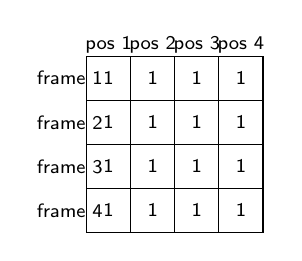
\begin{tikzpicture}[scale=.56]
\foreach \i in {0,...,3}{
  \foreach \j in {0,...,3}{
    \draw (\j,-\i) rectangle ++(1,-1);
    \node[font=\sffamily\scriptsize] at (\j+.5,-\i-.5) {1};
  }
}
\foreach \j/\x in {0/1,1/2,2/3,3/4}
  \node[font=\sffamily\scriptsize] at (\j+.5,.25) {pos \x};
\foreach \i/\x in {0/1,1/2,2/3,3/4}
  \node[font=\sffamily\scriptsize] at (-.38,-\i-.5) {frame \x};
\end{tikzpicture}
\par\tightnote{Latin4 exposure matrix $N$: 모든 cell이 정확히 1}
\end{center}

\subsection{집계와 실패 처리}

각 view의 raw text는 $[1,2,3,4]$의 순열 하나일 때만 유효하다. 설명문, 중복,
누락 숫자는 parse failure로 기록한다. 유효 $p_g$는 먼저 $C_g(p_g)$로
canonicalize한 뒤 hard vote한다. 최다 vote가 하나면 그것을 고르고, exact tie는
canonical permutation의 사전식 최소를 선택한다. token confidence는 최종
규칙에서 제거했다.

\subsection{전체 파이프라인}
\begin{center}
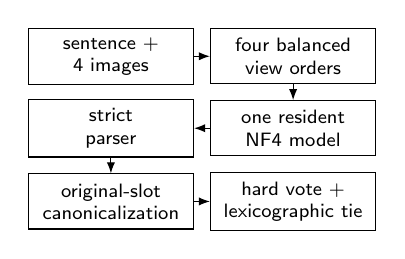
\begin{tikzpicture}[
  node distance=2mm,
  every node/.style={font=\sffamily\scriptsize},
  box/.style={draw,align=center,minimum width=21mm,minimum height=7mm},
  arr/.style={-{Latex[length=1.4mm]},thin}
]
\node[box] (x) {sentence +\\4 images};
\node[box,right=of x] (v) {four balanced\\view orders};
\node[box,below=of v] (m) {one resident\\NF4 model};
\node[box,left=of m] (p) {strict\\parser};
\node[box,below=of p] (c) {original-slot\\canonicalization};
\node[box,right=of c] (h) {hard vote +\\lexicographic tie};
\draw[arr] (x)--(v);
\draw[arr] (v)--(m);
\draw[arr] (m)--(p);
\draw[arr] (p)--(c);
\draw[arr] (c)--(h);
\end{tikzpicture}
\end{center}

\subsection{24 GB 배치 최적화}

단일 resident model, batch 1, SDPA, BF16 compute, sequential views를 사용했다.
adapter merge와 multi-model ensemble을 피했다. PyTorch allocator만으로는 driver
allocation을 놓치므로 model load 전부터 종료 후까지 NVML device-used memory를
0.5초 간격으로 측정했다. CUDA owner가 하나인지도 함께 감사했다.

\begin{tabularx}{\linewidth}{@{}lR{20mm}@{}}
\toprule
최종 819행 측정 & 값\\
\midrule
Views / parse failures & 3,276 / 0\\
Generation 평균 & 16.4693 s/row\\
Generation loop & 13,488.36 s\\
End-to-end & 13,990.46 s\\
Physical peak & 21.151\,GiB\\
GPU & RTX 3090 24\,GB\\
\bottomrule
\end{tabularx}
\end{multicols}

\newpage
\section{실험: 무엇을 남기고 무엇을 버렸는가}

\begin{minipage}[t]{0.57\textwidth}
\subsection*{최종 Q36 operational ablation (A)}
\begin{tabularx}{\linewidth}{@{}l c c r l@{}}
\toprule
모델 / checkpoint & views & 집계 & Public & 판정\\
\midrule
Q35--27B / 1073 & 4 & conf. & 0.92844 & fallback\\
Q36--27B / 1074 & 4 & conf. & 0.93019 & early probe\\
Q36--27B / 2726 & 4 & conf. & 0.92670 & 기각\\
\textbf{Q36--27B / 2726} & \textbf{4} & \textbf{hard} & \textbf{0.93542} & \textbf{최종}\\
Q36--27B / 2726 & 24 & hard & 0.93193 & 기각\\
Q36--27B / 3400 & 12 & hard & 0.93542 & 동점·고비용\\
\bottomrule
\end{tabularx}
\end{minipage}\hfill
\begin{minipage}[t]{0.40\textwidth}
\subsection*{Public score와 view 수}
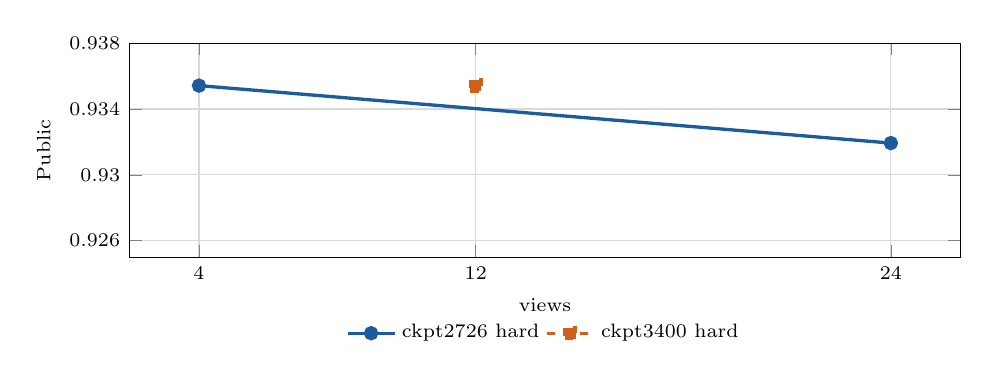
\begin{tikzpicture}
\begin{axis}[
  width=\linewidth,height=43mm,
  xmin=2,xmax=26,ymin=.925,ymax=.938,
  xlabel={views},ylabel={Public},
  xtick={4,12,24},
  ytick={.926,.930,.934,.938},
  yticklabel={\pgfmathprintnumber[fixed,precision=3]{\tick}},
  grid=major,grid style={black!15},
  tick label style={font=\scriptsize},
  label style={font=\scriptsize},
  legend style={font=\scriptsize,draw=none,at={(0.5,-.26)},anchor=north,legend columns=2}
]
\addplot[graphblue,very thick,mark=*] coordinates {(4,.93542) (24,.93193)};
\addlegendentry{ckpt2726 hard}
\addplot[graphorange,very thick,dashed,mark=square*] coordinates {(12,.93542)};
\addlegendentry{ckpt3400 hard}
\end{axis}
\end{tikzpicture}
\end{minipage}

\vspace{2pt}
\begin{multicols}{2}
\subsection{다섯 개의 정량 결론}

\begin{enumerate}
\item \textbf{모델 세대:} 동일한 4-view confidence 설정에서 Q36 early probe는
Q35 fallback보다 $+0.00175$였다. 단 checkpoint도 달라 세대의 순수 인과효과로
해석하지 않는다.
\item \textbf{step은 단조 축이 아님:} Q36 confidence는 step1074의 0.93019에서
step2726의 0.92670으로 하락했다.
\item \textbf{집계가 중요:} step2726에서 confidence를 제거한 hard vote가
$+0.00872$로 가장 큰 확인 개선이었다.
\item \textbf{view 추가는 역효과:} 같은 step2726 hard에서 4$\rightarrow$24
views는 $-0.00349$였다. pure-hard CSV는 16/819행에서 달랐다.
\item \textbf{추가 학습·추론 무이득:} step3400 TTA12는 최종과 동점이지만
학습 step과 per-row view가 모두 더 많다. 동점 시 더 작은 2726/Latin4를 채택했다.
\end{enumerate}

\subsection{개발 단계 clean954 ablation (B)}

\scriptsize
\begin{tabularx}{\linewidth}{@{}r c r c r r@{}}
\toprule
step & prec. & view & agg. & exact & s/row\\
\midrule
3000 & BF16 & 1 & hard & 229 & 1.537\\
3000 & NF4 & 1 & hard & 228 & 2.261\\
3500 & NF4 & 1 & hard & 227 & 2.313\\
3750 & NF4 & 1 & hard & 219 & 1.972\\
4000 & NF4 & 1 & hard & 212 & 1.977\\
4250 & NF4 & 1 & hard & 221 & 2.000\\
4292 & NF4 & 1 & hard & 223 & 2.023\\
3000 & NF4 & 4 & hard & 238 & ---\\
3000 & NF4 & 4 & conf. & 239 & same raw\\
4292 & NF4 & 4 & hard & 244 & 7.967\\
4292 & NF4 & 4 & conf. & 246 & same raw\\
\bottomrule
\end{tabularx}
\normalsize

\tightnote{Qwen3-VL--8B, image-disjoint 954행. checkpoint curve는 비단조였고
step4292에서 Latin4가 single-view보다 +21 exact였다. 이 패널은 모델·split이
다른 개발용 surrogate이므로 Q36 final accuracy로 환산하지 않는다.}

\subsection{12개 설계 질문 방어표}
\scriptsize
\begin{tabularx}{\linewidth}{@{}c Y Y c@{}}
\toprule
\# & 질문 & 관찰과 결정 & 증거\\
\midrule
1 & 더 최신 base? & Q36 early probe가 Q35 fallback보다 높음 & A\\
2 & 마지막 step? & 8B sweep 비단조; 2726/3400도 무개선 & A/B\\
3 & confidence? & 2726에서 $-0.00872$; 제거 & A\\
4 & 24 views? & Latin4보다 $-0.00349$; 제거 & A\\
5 & 12 views? & 더 긴 step과 함께 동점; 제거 & A\\
6 & position balance? & Latin4 exposure $N(i,j)=1$ & C\\
7 & parser 허용범위? & 3,276 views, failure 0 & A\\
8 & 24\,GB 적합? & peak 21.15\,GiB & A/C\\
9 & adapter merge? & unmerged NF4로 headroom 확보 & C\\
10 & ensemble? & 단일 checkpoint로 고정 & C\\
11 & 외부 API/data? & 학습·튜닝 사용 없음 & C\\
12 & 재현성? & model/adapter/source/CSV hash chain & C\\
\bottomrule
\end{tabularx}
\normalsize

\subsection{TTA 수렴과 계산량 (C)}
\tightnote{최종 Q36 test audit의 milestone 비교다. view가 늘수록 추가 예측 변화는
줄었지만 model-forward 시간은 거의 선형으로 증가했다. 점수는 제출된 4/24-view만
비교한다.}
\scriptsize
\begin{tabularx}{\linewidth}{@{}c R{18mm} R{20mm} c@{}}
\toprule
views & s/row & 직전 milestone 대비 변경행 & parse\\
\midrule
8  & 31.175 & --- & 0\\
12 & 46.735 & 10 & 0\\
16 & 62.216 & 7 & 0\\
20 & 78.278 & 4 & 0\\
24 & 93.843 & 1 & 0\\
\bottomrule
\end{tabularx}
\normalsize

\subsection{Vote agreement를 불확실성으로 사용 (B)}
\scriptsize
\begin{tabularx}{\linewidth}{@{}l R{17mm} R{18mm}@{}}
\toprule
4-view pattern & correct / rows & accuracy\\
\midrule
unanimous & 101 / 262 & 0.38550\\
3--1 & 79 / 308 & 0.25649\\
2--2 & 23 / 114 & 0.20175\\
2--1--1 & 38 / 216 & 0.17593\\
all different & 5 / 54 & 0.09259\\
\bottomrule
\end{tabularx}
\normalsize
\tightnote{8B clean954 진단이다. agreement가 낮을수록 정확도가 낮아,
label 없는 외부 데이터에서도 row-level uncertainty \textbf{표시}에는 쓸 수 있다.
정답 수정이나 threshold tuning에는 쓰지 않는다.}

\subsection{Split leakage audit (B)}
\scriptsize
\begin{tabularx}{\linewidth}{@{}l R{19mm} R{19mm}@{}}
\toprule
split & cross-set duplicate hashes & 영향 val rows\\
\midrule
clean954 dHash / byte & 0 / 0 & 0 / 0\\
same-seed random dHash & 1,495 & 584\\
same-seed random byte & 1,356 & 458\\
\bottomrule
\end{tabularx}
\normalsize
\tightnote{clean954는 image-disjoint 개발 판단을 위해 사용했고, contaminated random
split은 모델 승격에 사용하지 않았다.}

\subsection{해석의 경계}

여러 제출을 관찰했으므로 위 최대값에도 Public
overfitting 위험이 있다. 그래서 다음 원칙을 적용했다.
\begin{itemize}
\item 서로 다른 checkpoint, model, view 수가 함께 바뀐 행은 causal ablation으로
표현하지 않는다.
\item full-data Q36을 clean954로 채점하지 않는다.
\item 외부 팀 점수·레시피를 우리 성과나 근거로 포함하지 않는다.
\item Private, 현재 순위, 외부 데이터 성능은 \textbf{미지}로 남긴다.
\item 개별 test 정답을 역추정하거나 수동 수정하지 않는다.
\end{itemize}

\subsection{왜 최종은 2726/Latin4/hard인가}

최고 Public과 동률인 후보 중 학습 step, view 수, runtime, 규칙 복잡도가 가장
작다. 이 선택은 정답 label 없이도 적용 가능한 사전 규칙이며, 외부 평가에서
변경할 hyperparameter가 없다. 즉 \textbf{모델 크기}가 아니라
\textbf{계산 대비 정확도와 재현성}을 최적화한다.

\subsection{검증하지 못한 셀}

동일 Q36 checkpoint에서 rank8 대 rank32, 여러 seed, LoRA target 범위,
512 고정 정사각형 대 aspect-preserving pixel budget, 동일 checkpoint의 TTA12,
Private per-row error는 실행하지 않았다. 빈 셀을 유리한 추정치로 채우지 않는다.

\subsection{선택 규칙의 사전 고정}

최종 외부 평가에는 checkpoint-2726, Latin4, pure hard-majority,
lexicographic exact tie를 그대로 사용한다. 새 데이터에서 모델 선택, threshold
튜닝, 추가 학습, row-wise blending을 하지 않는다.
\end{multicols}

\newpage
\section{오류 분석, 일반화와 효율성}
\begin{multicols}{2}

\subsection{관찰 가능한 오류}

최종 test에는 label이 없으므로 semantic error를 정답처럼 단정할 수 없다.
대신 raw audit에서 관찰 가능한 실패를 세 계층으로 분리했다.

\begin{enumerate}
\item \textbf{형식 실패:} 유효 4-순열이 아닌 출력. 최종 3,276 view에서 0건.
\item \textbf{좌표 실패:} view label을 원본 slot로 잘못 옮김. permutation
round-trip test와 row audit로 차단.
\item \textbf{view 불일치:} canonical prediction들이 갈리는 경우.
hard vote가 이를 흡수하지만, tie는 정보 부족을 의미하므로 confidence를 새
정답 신호처럼 사용하지 않고 고정 사전식 규칙으로 끝낸다.
\end{enumerate}

남은 semantic 오류는 미세한 상태 변화, 반복 동작, 카메라 이동과 실제 사건 순서의
혼동, 문장과 시각 단서 충돌일 가능성이 있다. 이는 labeled external evaluation이나
사람이 정의한 error annotation이 있어야 검증할 수 있는 가설이다.

\subsection{일반화를 위한 선택}

\begin{itemize}
\item 입력 slot shortcut을 줄이는 deterministic shuffle
\item 좌표를 원상 복구한 뒤에만 집계하는 equivariant inference
\item 모든 position 노출을 최소 view로 균형화
\item confidence calibration에 의존하지 않는 hard vote
\item 단일 모델·단일 checkpoint·고정 parser
\item 외부 데이터에서 추가 학습·튜닝 금지
\end{itemize}

TTA24의 하락은 ``많은 변환 평균 = robustness''가 아님을 보여 준다. Latin4 이후
추가되는 view는 1차 균형을 개선하지 않으며, 품질이 낮은 view의 vote를 합칠 수 있다.

\subsection{한계와 위협}

\begin{itemize}
\item final Q36에 leakage-free labeled holdout이 없다.
\item Public을 여러 번 본 selection bias가 있다.
\item single seed이며 fold별 Q36 안정성을 측정하지 않았다.
\item semantic error category의 정량 annotation이 없다.
\item rank와 LoRA target의 독립 ablation이 없다.
\item Private와 외부 데이터 성능은 제출 전 알 수 없다.
\end{itemize}

따라서 ``SOTA''나 보이지 않은 데이터 성능을 주장하지 않고, 관찰된 end-to-end
점수와 재현 가능한 시스템 계약만 주장한다.

\columnbreak
\subsection{자원·지연시간 분석}

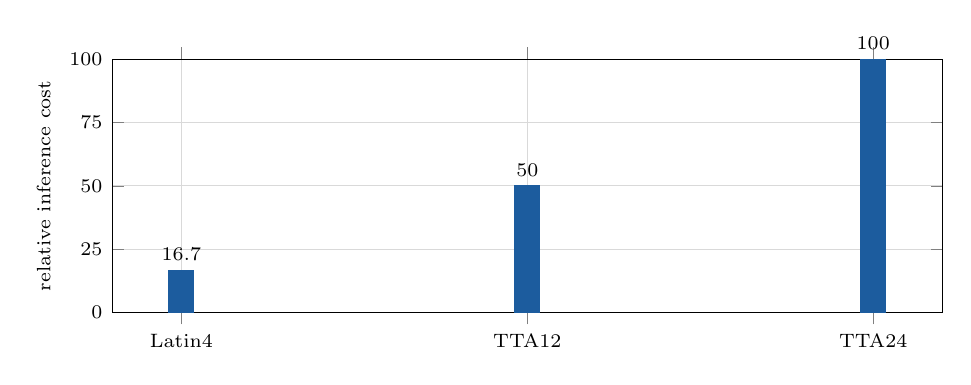
\begin{tikzpicture}
\begin{axis}[
  width=\linewidth,height=48mm,
  ybar,bar width=9pt,
  ymin=0,ymax=100,
  ylabel={relative inference cost},
  symbolic x coords={Latin4,TTA12,TTA24},
  xtick=data,
  ytick={0,25,50,75,100},
  grid=major,grid style={black!15},
  tick label style={font=\scriptsize},
  label style={font=\scriptsize},
  nodes near coords,
  every node near coord/.append style={font=\scriptsize}
]
\addplot[fill=graphblue,draw=graphblue] coordinates
  {(Latin4,16.7) (TTA12,50) (TTA24,100)};
\end{axis}
\end{tikzpicture}
\tightnote{동일 model의 view 수에 비례한 이론적 generation cost.
Latin4는 TTA24 대비 83.3\%를 절감한다.}

\begin{tabularx}{\linewidth}{@{}lR{22mm}@{}}
\toprule
항목 & 최종 실측\\
\midrule
GPU & RTX 3090 24\,GB\\
Physical peak & 21.15\,GiB\\
Peak headroom & 2.85\,GiB\\
Generation & 3.75 GPU-h\\
End-to-end & 3.89 h\\
Parse fallback & 0 rows\\
Models resident & 1\\
\bottomrule
\end{tabularx}

\subsection{구축 비용의 정직한 경계}

학습은 사비 RunPod RTX A6000, 최종 추론은 보유 RTX~3090에서 수행했다.
외부 상용 API 비용은 0이다. provider invoice, 전체 GPU-hour ledger, 로컬 전력과
감가상각이 하나의 검증된 receipt로 묶여 있지 않아 총액은 보고하지 않는다.
대신 재현 가능한 비용 지표인 step, view, wall time, peak memory를 제시한다.

\subsection{배포 설계}

\begin{tabularx}{\linewidth}{@{}Y Y@{}}
\toprule
선택 & 효과\\
\midrule
NF4 base + BF16 compute & 27B를 24\,GB에 적재\\
Unmerged adapter & base 중복·merge peak 회피\\
SDPA, batch 1 & 메모리 상한 단순화\\
Sequential Latin4 & 한 model로 4-view 처리\\
Strict parser & silent format corruption 방지\\
NVML sampler & allocator 밖 물리 사용량 포착\\
Atomic row audit & 중단 원인·집계 재검산\\
\bottomrule
\end{tabularx}

\subsection{보고서·코드 일치}

최종 보고서의 모든 수치와 설정은 \code{docs/final\_results.json}의 frozen
contract를 기준으로 한다. README의 final command와 wrapper default가 이 계약을
구현하며, 서로 다르면 preflight에서 중단한다.
\end{multicols}

\newpage
\section{재현성, 코드 검증과 결론}
\begin{multicols}{2}

\subsection{정확한 재현 절차}

\begin{enumerate}
\item 제공 데이터는 \code{data/train.csv}, \code{data/train/},
\code{data/test.csv}, \code{data/test/}에 둔다.
\item manifest로 pinned base 29개 파일과 15개 shard를 검증한다.
\item final adapter archive와 내부 tensor hash를 검증한다.
\item package preflight 후 frozen wrapper로 정확히 한 번 추론한다.
\item CSV schema와 raw audit 재집계를 독립 검증한다.
\end{enumerate}

{\scriptsize
\begin{verbatim}
python -B scripts/download_weights.py \
  --manifest configs/weights/qwen36-27b-final.manifest.json \
  --output models/Qwen3.6-27B
python -B scripts/download_final_adapter.py \
  --output weights/qwen36-checkpoint2726
python -B -m scripts.verify_evaluation_package
python -B -m scripts.run_final_inference \
  --data-dir data \
  --output-dir outputs/eval
\end{verbatim}
}

\subsection{Artifact provenance}
\begin{center}
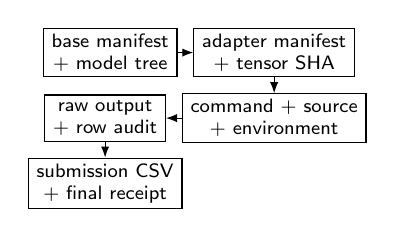
\begin{tikzpicture}[
  node distance=2mm,
  box/.style={draw,align=center,font=\sffamily\scriptsize,inner xsep=3pt,inner ysep=2pt},
  arr/.style={-{Latex[length=1.4mm]},thin}
]
\node[box] (m) {base manifest\\+ model tree};
\node[box,right=of m] (a) {adapter manifest\\+ tensor SHA};
\node[box,below=of a] (c) {command + source\\+ environment};
\node[box,left=of c] (r) {raw output\\+ row audit};
\node[box,below=of r] (s) {submission CSV\\+ final receipt};
\draw[arr] (m)--(a);
\draw[arr] (a)--(c);
\draw[arr] (c)--(r);
\draw[arr] (r)--(s);
\end{tikzpicture}
\end{center}

Base tree SHA는
\code{e4107e650879\ldots a207ec07}, adapter SHA는
\code{189f6c1be09b\ldots ca9f1f6}, 최종 CSV SHA는
\code{75c4c223cd73\ldots 29b7563}이다. 전체 값은 JSON manifest에 보존한다.

\subsection{검증자가 얻는 산출물}

\begin{tabularx}{\linewidth}{@{}lY@{}}
\toprule
\code{submission.csv} & 819행 canonical prediction\\
\code{audit.jsonl} & view order, raw text, parse, canonical vote\\
\code{metrics.json} & runtime, parse와 progress\\
\code{physical\_memory\_measurement.json} & NVML peak trace summary\\
\code{reproduction-receipt.json} & 모든 identity와 SHA chain\\
\bottomrule
\end{tabularx}

\subsection{동결 실행 환경}
\begin{tabularx}{\linewidth}{@{}lY@{}}
\toprule
Python / CUDA & 3.10 / 12.4\\
PyTorch & 2.6.0+cu124\\
Transformers & 5.13.1\\
PEFT / Accelerate & 0.19.1 / 1.7.0\\
bitsandbytes & 0.48.2\\
Attention / compute & SDPA / BF16\\
\bottomrule
\end{tabularx}

\tightnote{최종 raw run은 동일 네 view의 text와 canonical prediction을 보존했다.
제출용 pure-hard CSV는 그 audit에서 독립 재집계하고 SHA로 결합했다. 따라서
confidence 진단을 실행했다는 사실과 최종 hard aggregation을 혼동하지 않는다.}

\columnbreak
\subsection{주장--코드 추적표}

\begin{tabularx}{\linewidth}{@{}lY@{}}
\toprule
주장 & 구현·검증 위치\\
\midrule
index shuffle & \code{src/snuaichal/augmentation.py}\\
좌표 역변환·집계 & \code{src/snuaichal/tta.py}\\
strict Answer parser & \code{src/snuaichal/submission.py}\\
row/view audit & \code{src/snuaichal/inference.py}\\
물리 VRAM & \code{src/snuaichal/physical\_memory.py}\\
frozen command & \code{scripts/run\_final\_inference.py}\\
base·adapter 검증 & \code{scripts/verify\_evaluation\_package.py}\\
최종 수치 계약 & \code{docs/final\_results.json}\\
\bottomrule
\end{tabularx}

\subsection{외부 데이터 단일 실행 규약}
\begin{enumerate}
\item checkpoint-2726 adapter와 pinned base를 새로 선택하지 않고 그대로 사용한다.
\item CSV에 Answer가 있으면 CUDA model load 전에 거부한다.
\item Latin4/pure-hard 계약으로 정확히 한 번 inference한다.
\item raw audit에서 parser, canonicalization, vote와 CSV를 재계산한다.
\item 추가 학습·튜닝·row 수정·model mixing 없이 결과를 제출한다.
\end{enumerate}

\subsection{Release acceptance gate}
\begin{itemize}
\item model tree 29/29, safetensors shard 15/15
\item adapter manifest·tensor SHA 일치, non-finite 0
\item 819 IDs unique·canonical order, Answer domain $S_4$
\item 4 views/row, parse failure 0, unexpected CUDA process 0
\item report PDF A4 정확히 5쪽, 빌드 source와 PDF 동시 공개
\end{itemize}

\subsection{장점}

\begin{itemize}
\item 문제의 permutation symmetry를 학습과 추론 양쪽에 일관되게 반영
\item 네 view만으로 position balance를 수학적으로 증명
\item 더 많은 TTA·step·confidence가 실패한 결과까지 공개
\item 27B를 실제 24\,GB GPU에 배치한 물리 측정
\item 외부 평가에서도 바꿀 knob가 없는 단일 frozen pipeline
\end{itemize}

\subsection{결론}

최종 시스템은 가장 큰 계산을 택한 결과가 아니다.
\textbf{좌표 변환을 정확히 맞추고, 균형에 필요한 최소 네 view만 사용하며,
실제 24\,GB에서 재현되는 checkpoint-2726을 고정한 결과}다.
confidence 집계는 악화됐고, 24-view는 6배 계산에도 낮았으며, step3400/TTA12는
동점이었다. 이 실패를 포함한 ablation이 Latin4 hard-majority의 논리적·효율적
타당성을 방어한다.

외부 데이터에는 추가 학습 없이 동일 base, adapter, parser, Latin4와 집계를
그대로 적용한다. Private와 외부 점수는 미지로 남기되, 입력부터 CSV까지의
byte-level provenance로 운영진 실행과 제출 결과의 일치를 검증할 수 있다.

\subsection{참고문헌}
\scriptsize
\begin{enumerate}[label={[\arabic*]},leftmargin=1.7em]
\item T. Dettmers et al., ``QLoRA: Efficient Finetuning of Quantized LLMs,''
NeurIPS, 2023.
\item E. Hu et al., ``LoRA: Low-Rank Adaptation of Large Language Models,''
ICLR, 2022.
\item Qwen Team, ``Qwen3.6--27B model card,'' pinned revision documented in
the repository manifest, 2026.
\item SNUAICHAL, \code{docs/final\_results.json},
\code{docs/experiment\_log.md}, and repository source, frozen release.
\end{enumerate}
\normalsize

\subsection*{재현성 선언}
\tightnote{본 보고서는 우리 팀의 frozen artifacts만 사용한다. 타 팀의 점수나
비공개 레시피를 성과로 포함하지 않았으며, 알려지지 않은 Private·외부 성능과
실행하지 않은 실험을 추정하지 않았다.}
\end{multicols}

\end{document}
